\section{Optimal \textit{in silico} loading paths} \label{sec:optimalpaths}

	The most optimal loading path is the equibiaxial stress loading paths. This is not surprising as the equibiaxial stress response generally given very intuitive information on the mechanical response of soft tissues. Any odd number of loading paths will include the equibiaxial stress loading paths (Fig. \ref{fig:oddpaths}). Even when the number is even, we can observe that at least a few protocols are nearly equibiaxial in stress (Fig. \ref{fig:evenpaths}). For this reason, using an odd number of loading paths is highly recommended, as they will always include the minimal necessary set of loading paths, with the rest being average ratios in between (Fig. \ref{fig:oddpaths}). Even number of loading paths are generally very in consistent, and change slightly with each additional pairs of loading paths.  

%%%%%%%%%%%%%%%%%%%%%%%%%%%%%%%%%%%%%%%%%%%%%%%%%%%%%%%%%%%%
%-------------------	begin FIGURE 	-------------------%   
\begin{figure}
\centering
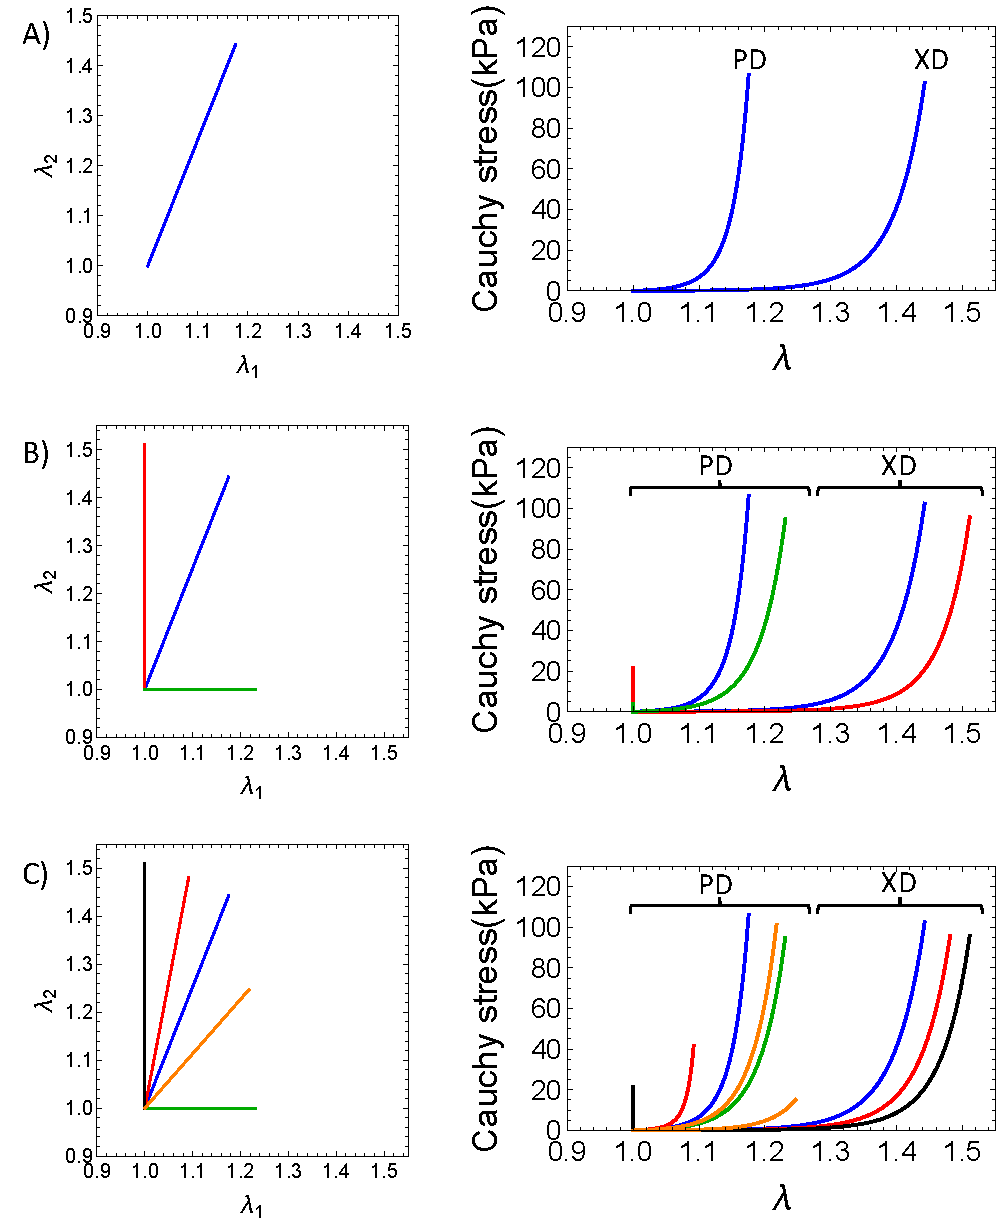
\includegraphics[width=\textwidth]{Images/chapter5/oddpaths}
\caption{The optimal loading paths for generating data for a given total odd number of paths as well as the associated mechanical response, which is consistently containing the equi-biaxial stress loading path and the loading paths at the boundary.}
\label{fig:oddpaths}
\end{figure} 
%-------------------	 end FIGURE 	-------------------%
%%%%%%%%%%%%%%%%%%%%%%%%%%%%%%%%%%%%%%%%%%%%%%%%%%%%%%%%%%%%


%%%%%%%%%%%%%%%%%%%%%%%%%%%%%%%%%%%%%%%%%%%%%%%%%%%%%%%%%%%%
%-------------------	begin FIGURE 	-------------------%   
\begin{figure}
\centering
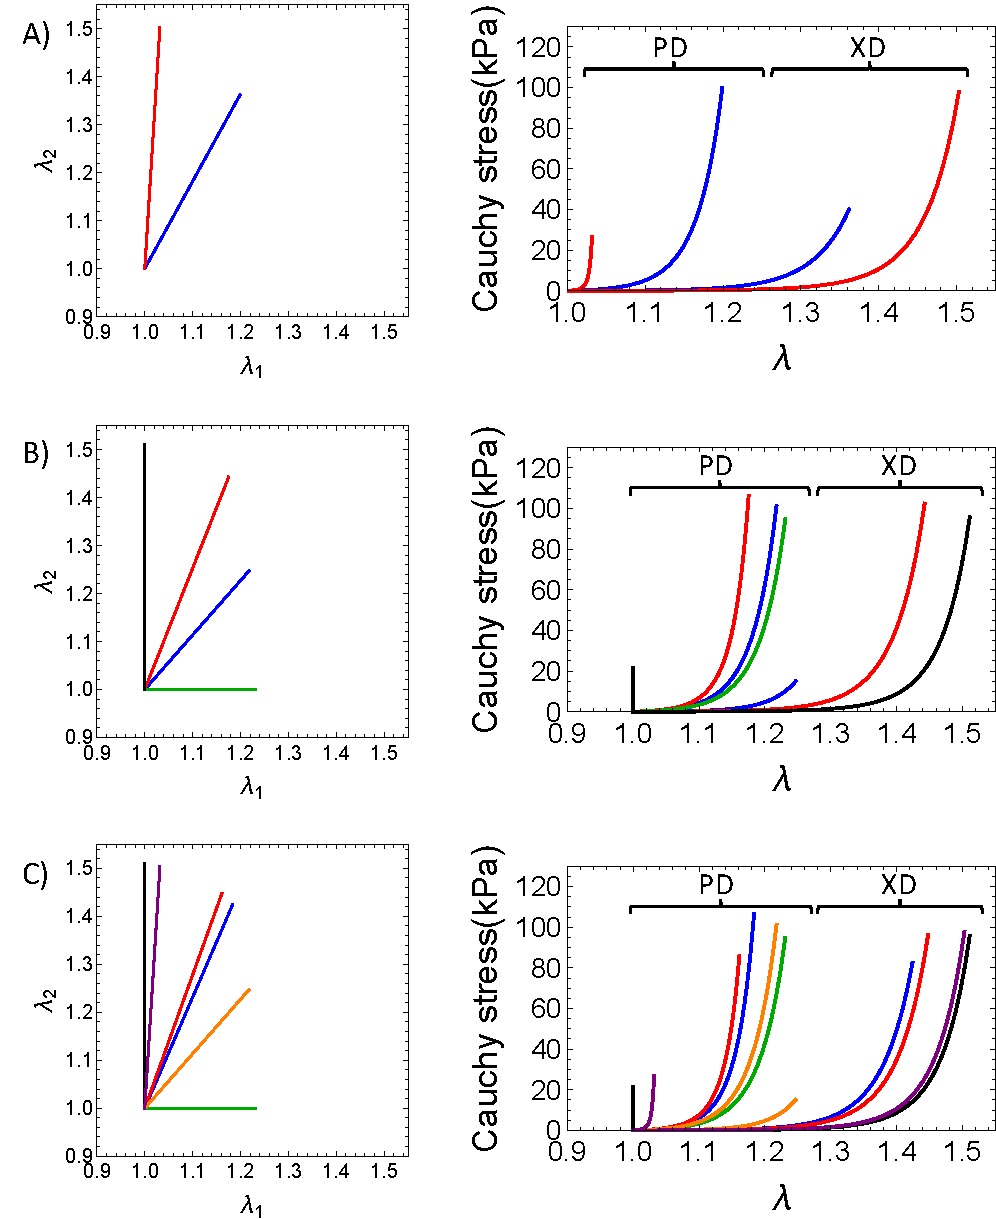
\includegraphics[width=\textwidth]{Images/chapter5/evenpaths}
\caption{The optimal loading paths for generating data for a given even total number as well as the associated mechanical response, which is much more unpredictable than the odd (Fig. \ref{fig:oddpaths}) but gravitates towards the boundaries and the equi-biaxial loading paths as the number increases.}
\label{fig:evenpaths}
\end{figure} 
%-------------------	 end FIGURE 	-------------------%
%%%%%%%%%%%%%%%%%%%%%%%%%%%%%%%%%%%%%%%%%%%%%%%%%%%%%%%%%%%%